\chapter{LOCAL MOTOR INVARIANT}
\label{chap:li}

\nomenclature[f1]{$G$}{A Lie Group}
\nomenclature[f2]{$g_a$}{an element in Lie Group $G$ with parameter $a$}
\nomenclature[f3]{$I(x)$}{Invariant Function of $x$}
\nomenclature[f4]{$\ep$}{The parameter of a lie group element}
\graphicspath{{LocalInvariant/LocalInvariantFigs/EPS/}{LocalInvariant/LocalInvariantFigs/}}
For animals,  being able to maintain the global motor invariant is not enough.
For a fish, preserving \emph{Global Motor Invariant}  means the swimming can be sustained and stable.
But a fish also needs to adjust the swimming speed and swimming direction,which is of crucial importance for survival.
In real-life, animal can  motion primitive according its purpose with precision.
This chapter develops the control strategies for tweaking motion patterns according to motion purpose.

It is important to remember that such tweaking strategies are severely constrained by the computation and memory capacity of neural system,  and should resemble  motion primitive in exploring natural dynamics.
For \cms, it is of no meaning developing walking pattern by exploring natural dynamics but use optimization to adjust the walking speed. To meet such requirements, \moit adopted a combination of ideas.

At first, when tweaking motion patterns, stability should not be violated. 
As stated in the previous chapter, a topology conjugation (one-one continuous invertible mapping)maintains the topology thus maintains the qualitative stability. Thus the ``tweaking'' action should be a topology conjugation. In an alternative perspective, such operations form a group and permit a combination operation. 
For motor control, this means if two tweaking actions preserve the stability separately, combination of the two actions also preserve the stability.
The space of topology conjugation is very large, \moit only investigate a subset that is biological supported and computational efficient: \emph{The Lie Transformation Group}.
Selected groups can be divided into orthodox subgroups , each of which is continuous and can be parametrized by one parameter.
In \cms, such parameters close related to motion purpose or requirement, for example, walking speed or swimming direction.

From dynamic perspective, ``tweaking''  should also explore natural dynamics (passive based) as primitives.
Methods adopted in \moit belongs to  a popular passive-based control principle, which carries many names: Controlled Symmetry, Controlled Lagrange, or Potential Shaping.
Different names reflect the fact that this method can be developed through different ways.
Roughly speaking, the original dynamic system is transformed according to motion purpose, the kinematics is untouched and control is applied by modifying the potential energy.
Such methods suit biological actuators like muscles and are also computational efficient:
Closed form formula are developed for converting tweaking parameters to control effort.

This chapter is lay out in this way:
Section~\ref{sec:groupandsymmetry} introduces the basic idea of group and symmetry from intuitive geometry examples to more abstract algebraic formulation. Section~\ref{sec:liecontrol} investigate application of controlled Lagrange method.
At last a simple dynamic example is provided in Section~\ref{sec:symball}.

Group and Invariant are the two sides of a coin.
Group are defined by invariant.
Deciding which group should be applied to motion is equivalent finding which invariant should be persevered.
The quantitative property preserved are called \emph{Local Motor Invariant}.







\section{Group and Symmetry}
\label{sec:groupandsymmetry}
%To make motions realistic, some natural looking features should also be preserved.
%Some features of motions such as smoothness or energy efficient are quantitative.
%\cms research should provide a framework preserving feature.
%Another question mission is animals can finish motion tasks require high accuracy.
%
%These are the motivations for the development of \emph{Local Motor Invariant}.
%Local Motor Invariants are quantitative properties of motions, the idea of invariant preserving are abstracted as the ``Symmetry'' and Group theory.
%Features are modelled as symmetrical functions, while feature preserving actions form a group.
%From dynamic perspective, motions are solutions to dynamic equations.
%The actions transform one motion to another close related to the Lie Group Theory for differential equations\citep{olver1986applications}.
%
%The introduction of Lie Group not only provides a powerful mathematical tools for modelling the symmetry property, but also provides an idea to simplify the solving the dynamics.



For the more traditional geometrical perspective, ''Symmetry''  means a geometry is the same after certain transformation.
For the example, a square remains the same after  $90$ degree clockwise rotation, as shown in Figure~\ref{fig:symsquare}.
\begin{figure}[!htbp]
  	\begin{center}
   	\includegraphics[width=0.7\textwidth]{Symmetry}
	\end{center}
	\caption{Symmetry of The Square}
    \label{fig:symsquare}
\end{figure}

Actions that preserve the square shape have some properties.
For example, if the action of $90$ degree clockwise rotation preserves the shape, so will the action of rotating twice, that's $180$ degree clockwise rotation.

All the action that can preserve the symmetry form a group $G$.
A group has the following properties.
\begin{enumerate}
\item For any $g_a,g_b$ in $G$, \,$g_a*g_b$\, belongs to $G$. (The operation ``$*$'' is closed).

\item For any \,$g_a,g_b,g_c\in G$, \,$(g_a*g_b)*g_c=g_a*(g_b*g_c)$. \,(Associativity of the operation).

\item There is an element $e\in G$ such that \,$g_a*e=e*g_a=g_a$\, for any \,$g_a\in G$. (Existence of identity element).

\item For any \,$g_a\in G$\, there exists an element $g_h$ such that \,$g_a*g_h=g_h*g_a=e$. \,(Existence of inverses).
\end{enumerate}

For the square example, all the actions preserve the same form the group $G$.
$g_1$ is  $90$ degree clockwise rotation, identity element $e$ is no rotation,
$g_2=g_1*g_1$ is rotate $90$ degree clockwise twice.
Since $g_2$ preserve symmetry, $g_2$ is a element of the group $G$, 


From algebraic perspective, ``Symmetry'' means the value of function is invariant after transformation.
For a function $I(x)$,
The group transformation is define by $\tilde{x}=g_a(x)$
By symmetry, we mean $I(x)=I(\tilde{x})$.
$I(x)$ is an invariant function of group $G$.


Note that  shapes invariant by actions in $G$ is not unique.
Many shapes are invariant, and their combinations are also invariant, as shown in Figure~\ref{fig:SymmetrySpace}. 
In algebraic sense,  invariant functions of group $G$ form a space, the invariant space $I^G$.


\begin{figure}[!htbp]
  \begin{center}
    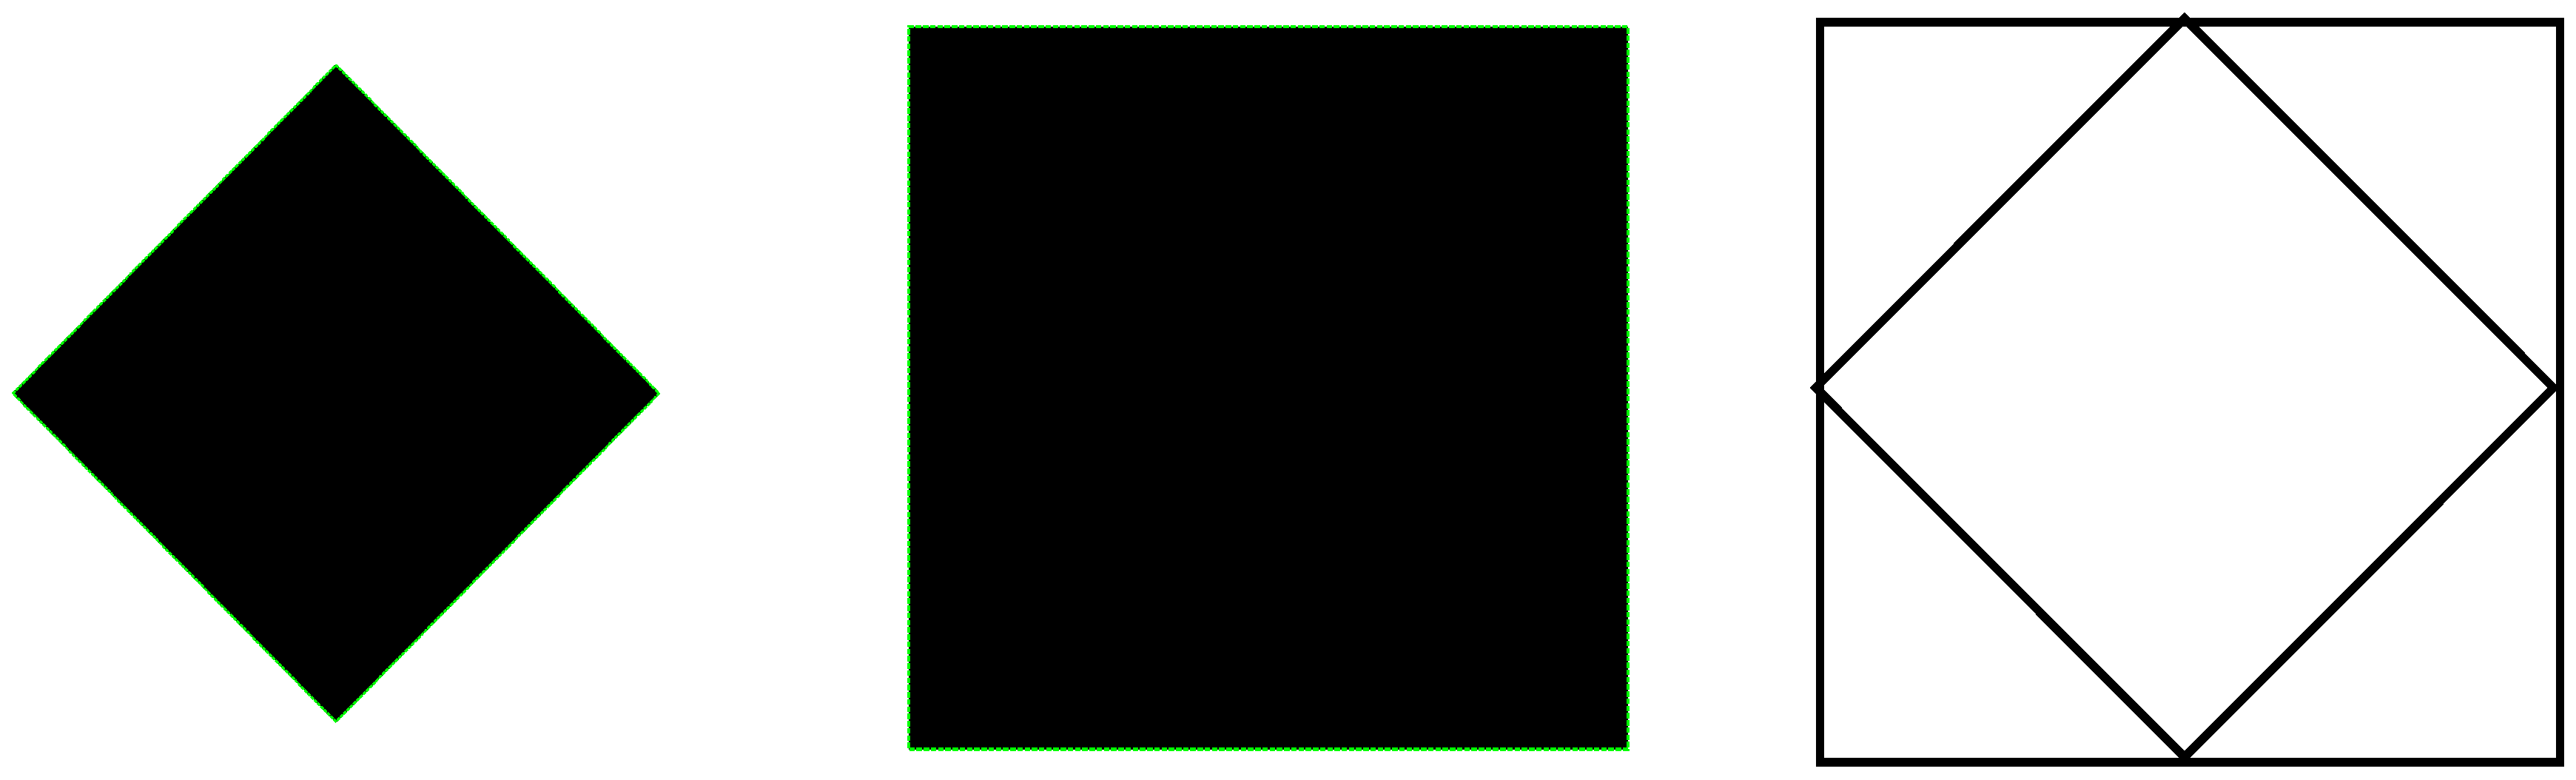
\includegraphics[width=0.7\textwidth]{SymmetrySpace}
    \caption{Two invariant Shapes and the invariant combination}
    \label{fig:SymmetrySpace}
\end{center}
\end{figure}

\subsection{Lie Group and Differential Equation}
Physically-based motions are usually described by differential equations, and motion is the solution of the equation.
As the square shape, there are also symmetry groups that keep the differential equations invariant.
For differential equations, the important property is elements in such group can transform one solution into another\citep{olver1986applications}.
For \cms, this property potential can help reduce computational burden, new motions can be achieved through applying group transformation to motion primitives.




Simply put, \emph{Lie Group} is continuous group, which is also a manifold.
Since it is a manifold, coordinate system can be assigned to a Lie Group and each elements can be parametrized.
For example,the symmetry rotation group of square is discrete,while symmetry group of circle is continuous.
For the symmetry group of the circle, each element can be parametrize by the the rotation angle.
In the following discussions, for each group element $g$, $\ep$ is the parameter.

Theory of Lie group comes from the study of differential equations.
For a differential equation in Equation~\ref{eq:difforg}.
\begin{equation}
\label{eq:difforg}
\dot{\state}=F(\state)
\end{equation}
Invariant function $I$ can be defined as:
\[
I(t,\state,\dot{\state})=F(\state)-\dot{\state}
\]
Solutions of the differential equation are the kernel of the invariant function $I$ :
 \[
 I(t,\state,\dot{\state})=0
 \]
 
 
The group transformation will act on all the variables of invariant function, so $t$,$\state$ and $\dot{\state}$ are all transformed.
\[
(t,\state,\dot{\state}) \mapsto (\tilde{t},\tilde{\state},\dot{\tilde{\state}})
\]
If the group $G$ is symmetrical, then value of the  function $I$ will be invariant.
Thus kernel are transformed into kernel, and transformed variables are still solutions to the original differential equations. 
\[
I(t,\state,\dot{\state})=I(\tilde{t},\tilde{\state},\dot{\tilde{\state}})=0
\]


Note that the $\dot{\state}$ is not independent, it depends on the $t$ and $\state$,
\[
\dot{\tilde{\state}}=\frac{d \tilde{\state} }{d \tilde{t}}
\]
From geometrical perspective, it is not easy to present  transformation of $t$.
Instead, we define two actions on the state space and tangent space.
In the state space, we define the  action $g$ that transform the state. 
\[
g(\state)=\tilde{\state}
\]
In the tangent space, we define the \emph{lift action} $Tg$ 
\[
Tg(\dot{\state})=\dot{\tilde{\state}}
\]

$Tg$ can be worked out by formatting the derivatives in original coordinate system.
For example, the translation $g_{\ep}$ 
\[
(x,y)\mapsto (x+\ep,y+\ep)
\]
$Tg_{\ep}$ is
\[
(\dot{x},\dot{y}) \mapsto (\dot{x},\dot{y})
\]
$Tg$ is the identity element $e$.


In the general cases, $g$ transform Equation~\ref{eq:difforg} into Equation~\ref{eq:trdiff}
\begin{equation}
\label{eq:trdiff}
Tg(\dot{\state})=F(g(\state))
\end{equation}
if $g$ is symmetrical, Equation~\ref{eq:difforg} and Equation~\ref{eq:trdiff} are equivalent







 	
For example, 
The scaling action is applied to the state space of the mass spring system of Equation~\ref{eq:stateform}. 
\[
\tilde{\state}=g_{\ep}(\state)=[\ep q, \ep \qd ]
\]
then the lift action is
\[
\tilde{\state}=Tg_{\ep}(\state)=[\ep \qd, \ep \ddot{q}]
\]



by substitution $\state \mapsto \tilde{\state}$, the original system become
\[ 
\dot{\tilde{\state}}=
\left[ 
\begin{array}{cc}
0 &1\\
-1 &0 
\end{array}
\right]\tilde{\state}
\]
which is 
\begin{equation}
\label{eq:tranmas} 
\ep \dot{\state}=
\left[ 
\begin{array}{cc}
0 &1\\
-1 &0 
\end{array}
\right]\ep \state
\end{equation}

Equation ~\ref{eq:tranmas} is equivalent to  Equation~\ref{eq:stateform}.
If $\state(t)$ is a solution, so is $\tilde{\state}(t)$.

To verify the group property. define $*$ as:
\[
g_{\ep_1}*g_{\ep_2}(\state)=[\ep_1 \ep_2 q, \ep_1 \ep_2 \qd]
\]

The inverse is:
\[
g_{\ep}^{-1}=g_{\frac{1}{\ep}} \;\ep \in R^+
\]

\begin{mydef}
For a group $G$, the invariant function of state $I(\state)$ is called \emph{local motion invariant} of $G$. 
\end{mydef}

Invariant functions $I(\state)$ has important  meaning in dynamics. 
According  \textbf{Noether's Theorem}, each $I(\state)$ corresponds to a conservative law. 


\section{Lie Group and Controlled Lagrange}
\label{sec:liecontrol}
Motions Adaptation might not only explore symmetry groups of natural dynamics.
In real-life, animals will execute control effort for adapt motions; also For a dynamic system, working out the symmetry group might be an non-trivial task.
In \cms, it is possible the desired quantitative properties is not an invariant of the natural dynamics.
For this end, \emph{Control Symmetry} is proposed.
Based on biological research foundlings\citep{flash2007affine}, some simple group are assigned as the symmetry group of the motor dynamics system first.
The control effort are applied to ensure the symmetry.


Usually the natural dynamics are presented as by Euler-Lagrange Equation~\ref{eq:uncontrolled_euler_lagrange}\citep{Goldstein2002}.
\begin{equation}
\frac{d}{dt} \frac{\partial L}{\partial \qd} - \frac{\partial L}{\partial q} = 0
\label{eq:uncontrolled_euler_lagrange}
\end{equation}

Where $L=K-V$, $L$ is the Lagrange, $K$ is the kinetic energy, $V$ is the potential energy,$q$ is the generalized coordinates, and $\qd$ is the generalized velocity.

From the symmetry perspective,transformed equation of $g$ is Equation~\ref{eq:liegroup_euler_lagrange}, for the control perspective, the controlled dynamics is Equation~\ref{eq:controlled_euler_lagrange}. If symmetry is persevered, the two equation should be equivalent, then symmetry control input $\ulocal$ can be calculated.
\begin{align}
\frac{d}{dt} \frac{\partial L}{\partial \dot{\tilde{q}}} - \frac{\partial L}{\partial \tilde{q} }&=0,\label{eq:liegroup_euler_lagrange}\\
\frac{d}{dt} \frac{\partial L}{\partial \qd} - \frac{\partial L}{\partial q}&=\ulocal. \label{eq:controlled_euler_lagrange}
\end{align}





The group we assigned are homogeneous or affine group, this mainly because two reasons:
\begin{itemize}
\HiItem{Biological Reason} Homogeneous and affine group close related to the vision system, which serve the foundation of navigation and perception.
\HiItem{Application Reason} Both the group elements and transformed equations are easy to compute, this will make planning and control  computational efficient.
\end{itemize}

Several groups are shown in below:

\subsection*{ Offset Action}
The offset action will modify the coordinate by a constant, speed and time will be unchanged.
\[
(t,q,\qd) \mapsto (t,q+\ep,\qd)
\]
The state transformation and lift action are
\begin{align}
\goff(\state) &= [q+\ep,\qd] \\
T\goff(\dot{\state})&=\dot{\state}=[\qd,\qdd]
\end{align}
on phase space, if $q$ is the horizontal axis, and $\dot{q}$ is the vertical axis, offset the effect of moving the phase plot horizontally~\ref{fig:goff}.

\begin{figure}[!htbp]
  \begin{center}
      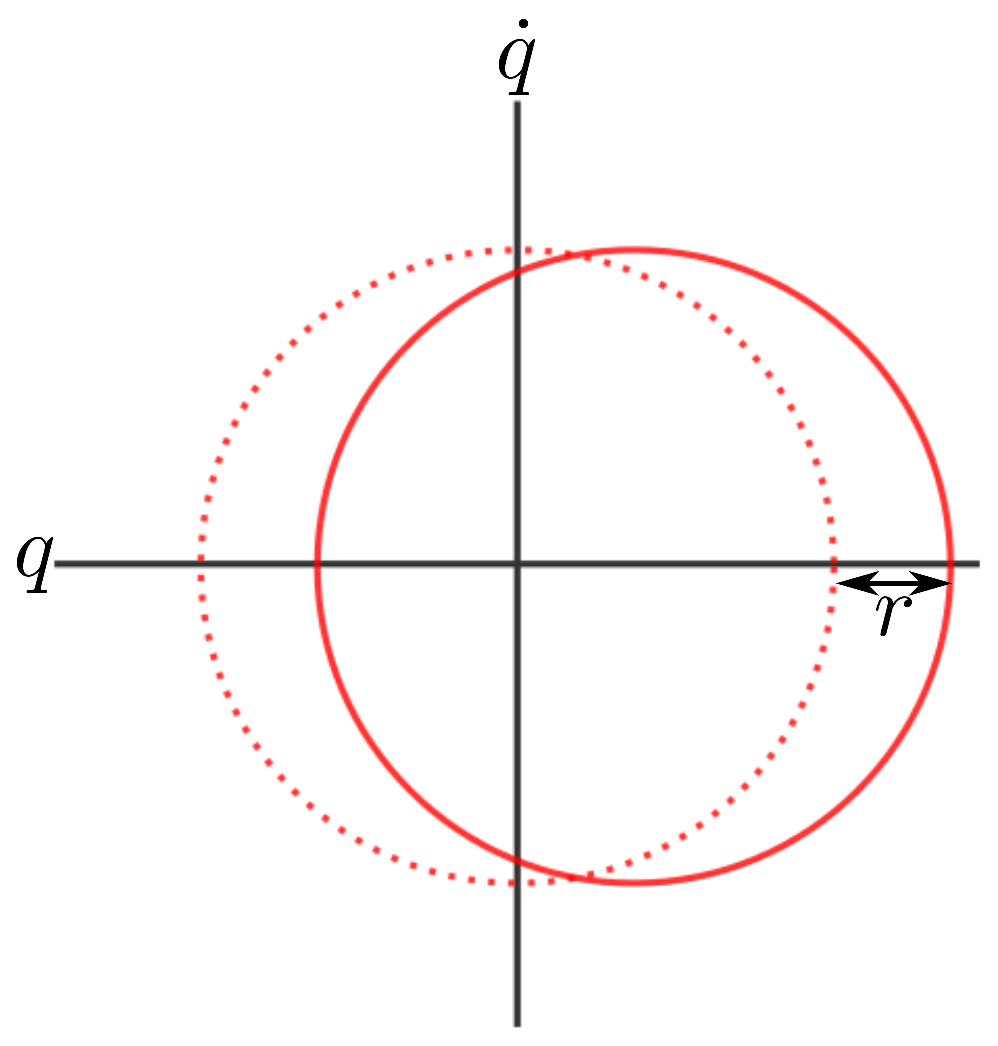
\includegraphics[width=0.7\textwidth]{g_off}
    \caption{Offset Action}
    \label{fig:goff}
\end{center}
\end{figure}

Substituted the transformed $q$ and $\qd$ into Equation~\ref{eq:liegroup_euler_lagrange} and Equation~\ref{eq:controlled_euler_lagrange}.
The symmetry control input
\begin{equation}
\ulocal(q) = \frac{\partial}{\partial q} \left(V(q)-V(\tilde{q}) \right).
\end{equation}

For example, the transformed equation and control equation are as follows.
\begin{align}
\ddot{\tilde{q}}+\tilde{q}-\ep&=0 \nonumber \\
\ddot{q}+q&=\ulocal \nonumber
\end{align}

The local control input is
\[
\ulocal(q)=\ep
\]




\subsection*{Time Scaling}

%g_st(q,dot{q})=(q,st*dot{q})
Time scaling will scale down the time variable, coordinates are kept. speed are scale up.

\[
(t,q,\qd) \mapsto (\frac{t}{\ep},q,\ep \qd)
\]

The correspond state transformation and lift action are
\begin{align}
\gts(\state)&=[q,\ep \qd] \nonumber \\
T\gts(\dot{\state})&=[\ep \qd,\ep^2 \ddot{q}]\nonumber
\end{align}

Then the local control is 
\begin{equation}
\ulocal(q) = (1-\ep^2) \frac{\partial V(q)}{\partial q}.
\end{equation}

For example, for the mass spring system,transformed and controlled equations are

\begin{align}
\frac{\ddot{\tilde{q}}}{\ep^2}+q&=0 \nonumber \\
\ddot{q}+q&=\ulocal \nonumber
\end{align}
The local control input is:
\[
\ulocal=(1-\ep^2)q
\]

\begin{figure}[!htbp]
  \begin{center}
    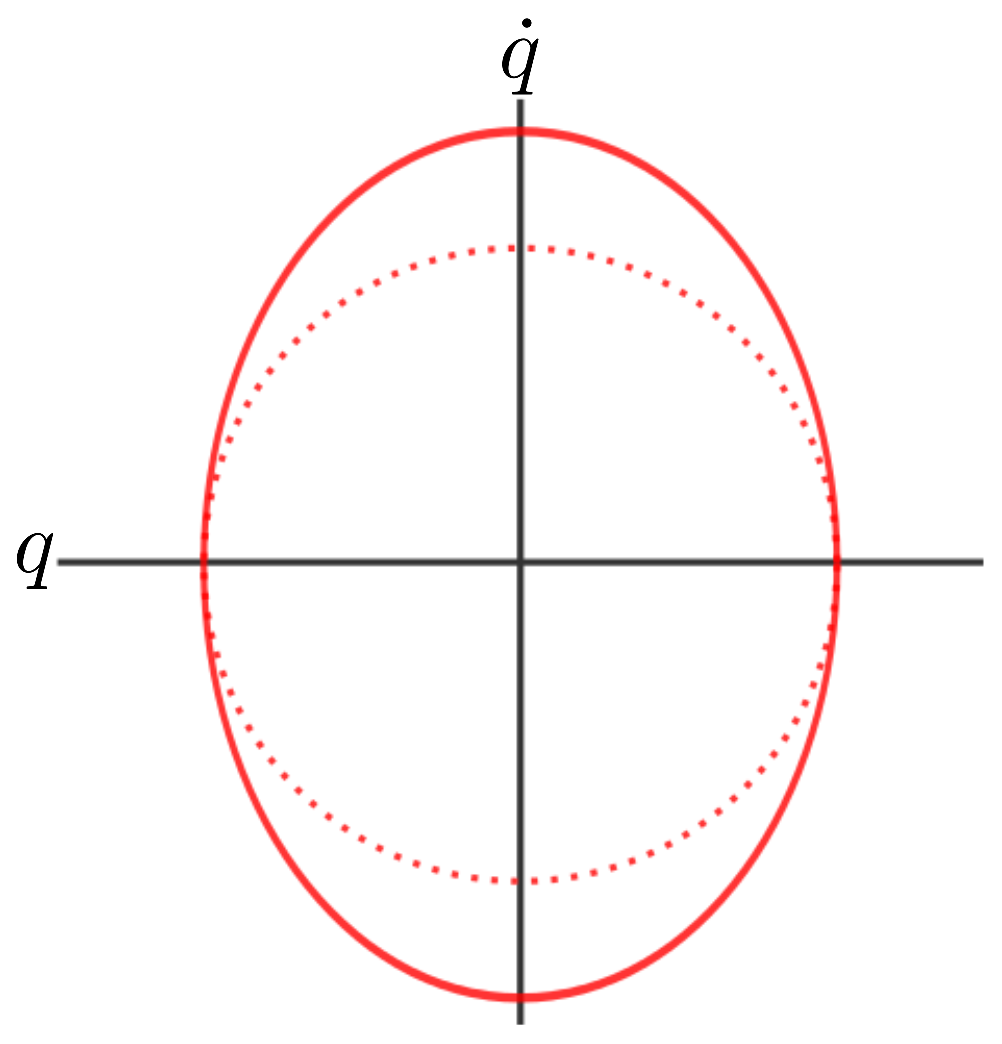
\includegraphics[width=0.7\textwidth]{g_ts}
	 \caption{Time Scaling Action}
    \label{fig:gts}
\end{center}
\end{figure}


\subsection*{Energy Scaling}
For some system moving the the conservative field.
The energy is preserved and different motion present different level of energy.
For such system, we have the energy $E(\state)=K+V$, where $K$ is the kinetic energy,
$V$ is the potential energy.
\[
E(\tilde{\state})=\ep^2 E(x)
\]
To generalize uniformly
\begin{align}
K(\tilde{\state})=\ep^2 K(\state) \nonumber\\
V(\tilde{\state})=\ep^2 V(\state) \nonumber
\end{align}


If the mass of system is constant, energy scaling can be achieved by linear transformation.
\[
(t,q,\qd ) \mapsto ( \frac{f(\ep)}{\ep}t ,f(\ep)q,\ep\qd)
\]
$f(\ep)$ is a function of $\ep$, which is determined by the conservative force.
On phase plot, this has the effect enlarge the phase portrait,as show in Figure~\ref{fig:gen}.
\begin{figure}[!htbp]
  \begin{center}
      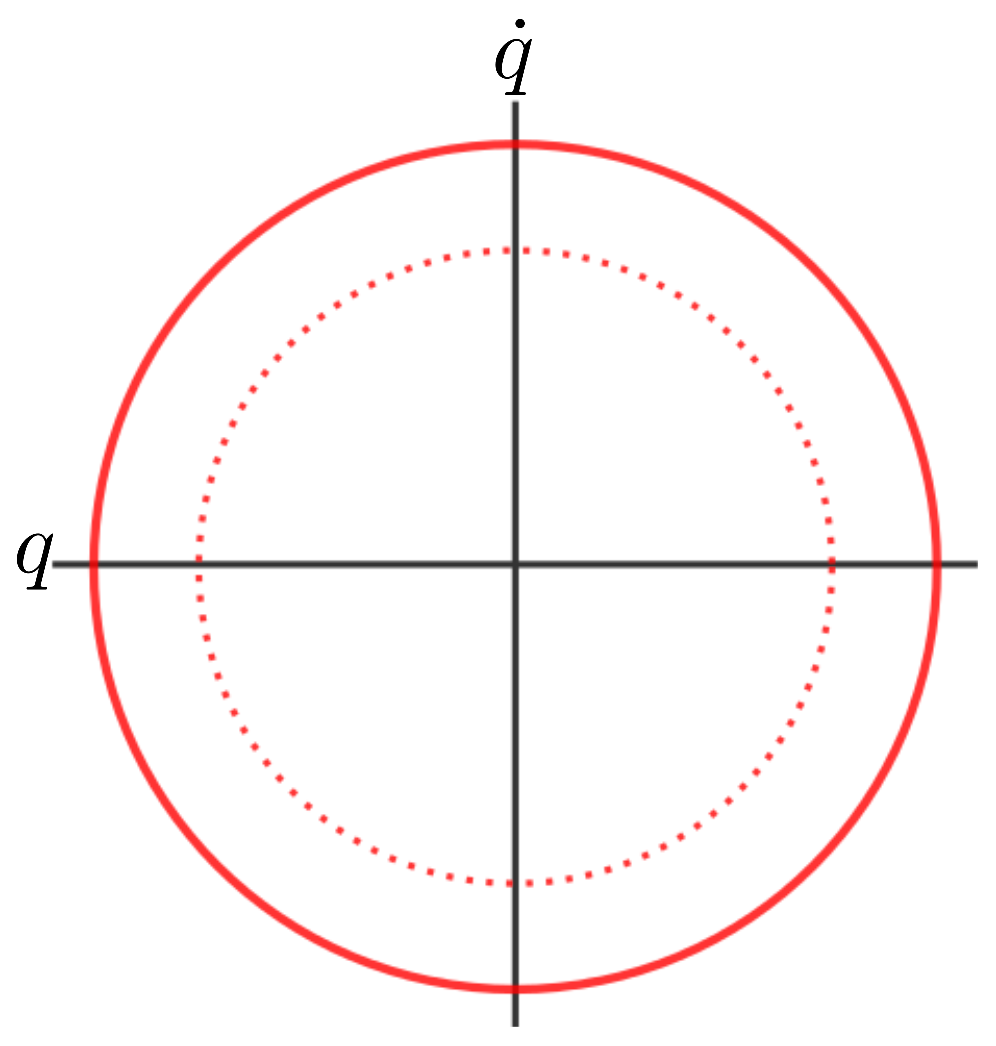
\includegraphics[width=0.7\textwidth]{g_en}
    \caption{Energe Scaling Action}
    \label{fig:gen}
\end{center}
\end{figure}

The state transformation and lift action
\begin{align}
\gen(\state)&=(f(\ep) q,\ep \dot{q}) \nonumber\\
T\gen(\dot{\state})&=(\ep \dot{q},\frac{\ep^2}{f(\ep)}\qdd)
\end{align}
$\ulocal$ can be developed by applying the pos scaling and time scaling in a combined manner.



For the mass spring system , $E=\frac{1}{2}(q^2+\qd^2)$,$f(\ep)=\ep$, and because the energy scaling is kept by the original system, we have
\[
\ulocal=0
\]



\subsection*{Time Offset}
we can also offset the time $t$
\[
(t,q,\qd) \mapsto (t+\ep,q,\qd)
\]

For dynamic system, Time offset symmetry is preserved by any system.
For system with limit cycle, Time offset has a special effects like phase modification.
On phase plot, this has the effect rotate on the limit circle about an angle, as shown in Figure~\ref{fig:gtoff}.
\begin{figure}
  \begin{center}
      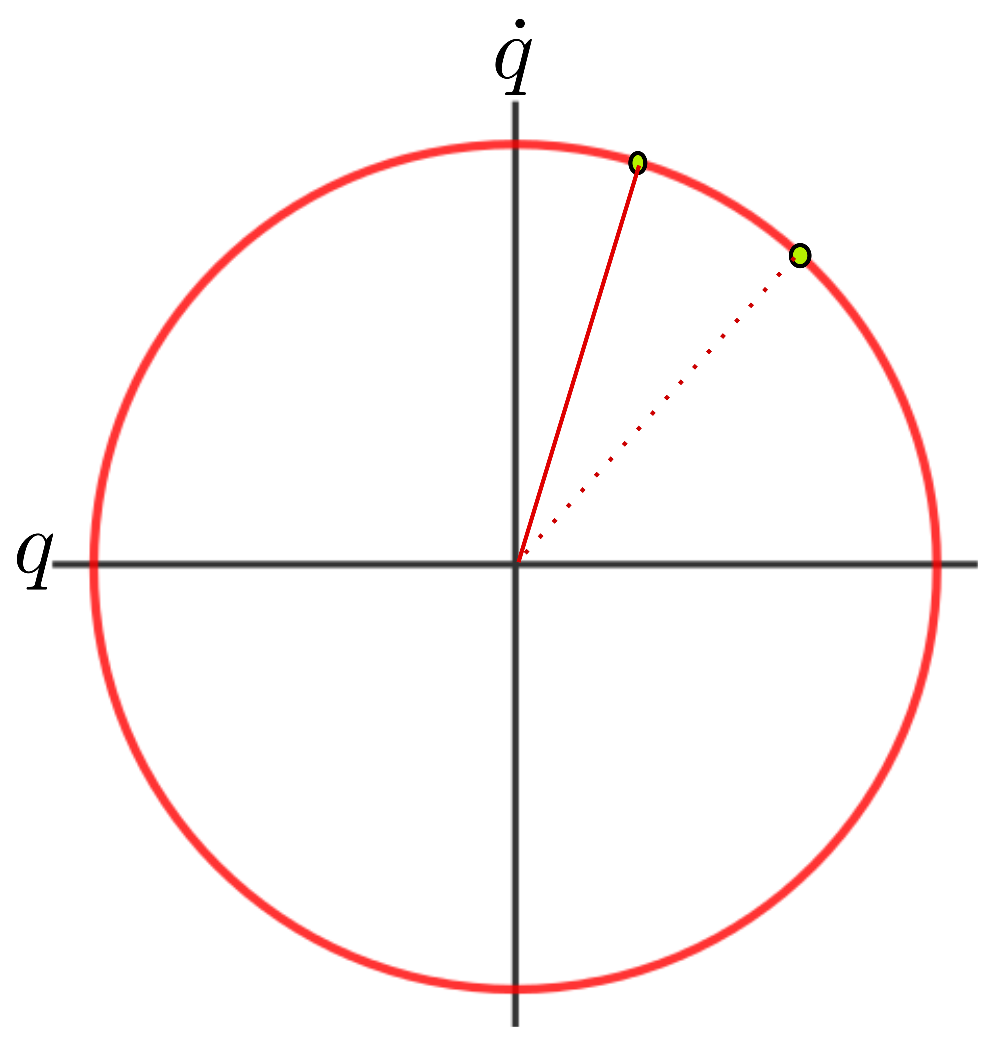
\includegraphics[width=0.7\textwidth]{g_toff}
    \caption{Offset Action}
    \label{fig:gtoff}
\end{center}
\end{figure}





\section{Example:Bouncing Ball dropped from Different Height}
\label{sec:symball}
Even it is a hybrid system,
The bouncing ball system has a energy scaling symmetry.

the energy function 
\[
E=\mathrm{g}q+\frac{1}{2}m\qd^2
\]
then
\[
f(\ep)=\ep^2
\]
the energy scaling transformation is
\[
\gen(\state)=[\ep^2 q, \ep \qd]
\]

Given the motion of a ball dropt at $5$,shown in Figure~\ref{fig:bouncing5},set $\ep=\sqrt{2}$, through transformation, motion dropped from $10$ are shown in Figure~\ref{fig:bouncing10}
\begin{figure}[!htbp]
  \begin{center}
      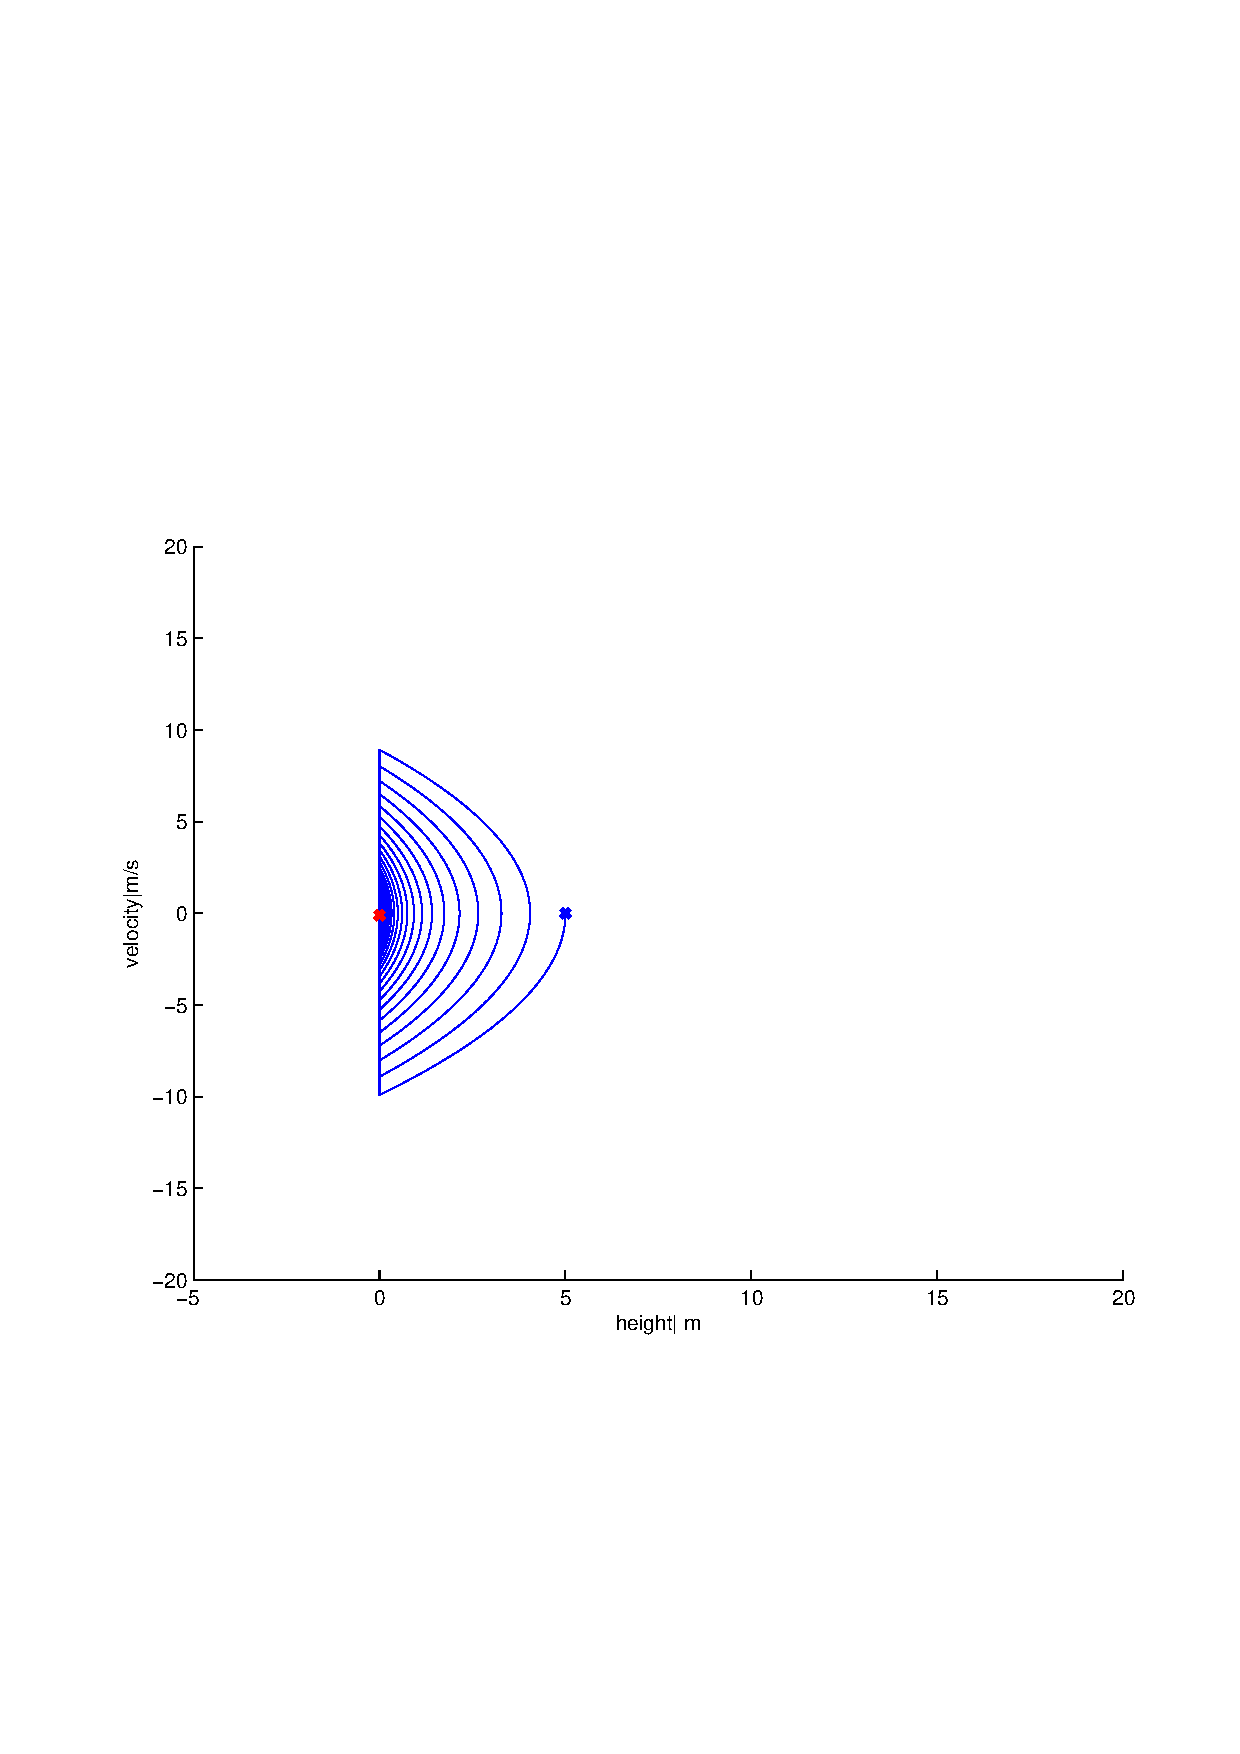
\includegraphics[width=0.7\textwidth]{BouncingBallPhasePlotuncontrolledDropAt5}
    \caption{Drop at 5}
    \label{fig:bouncing5}
\end{center}
\end{figure}


\begin{figure}[!htbp]
  \begin{center}
      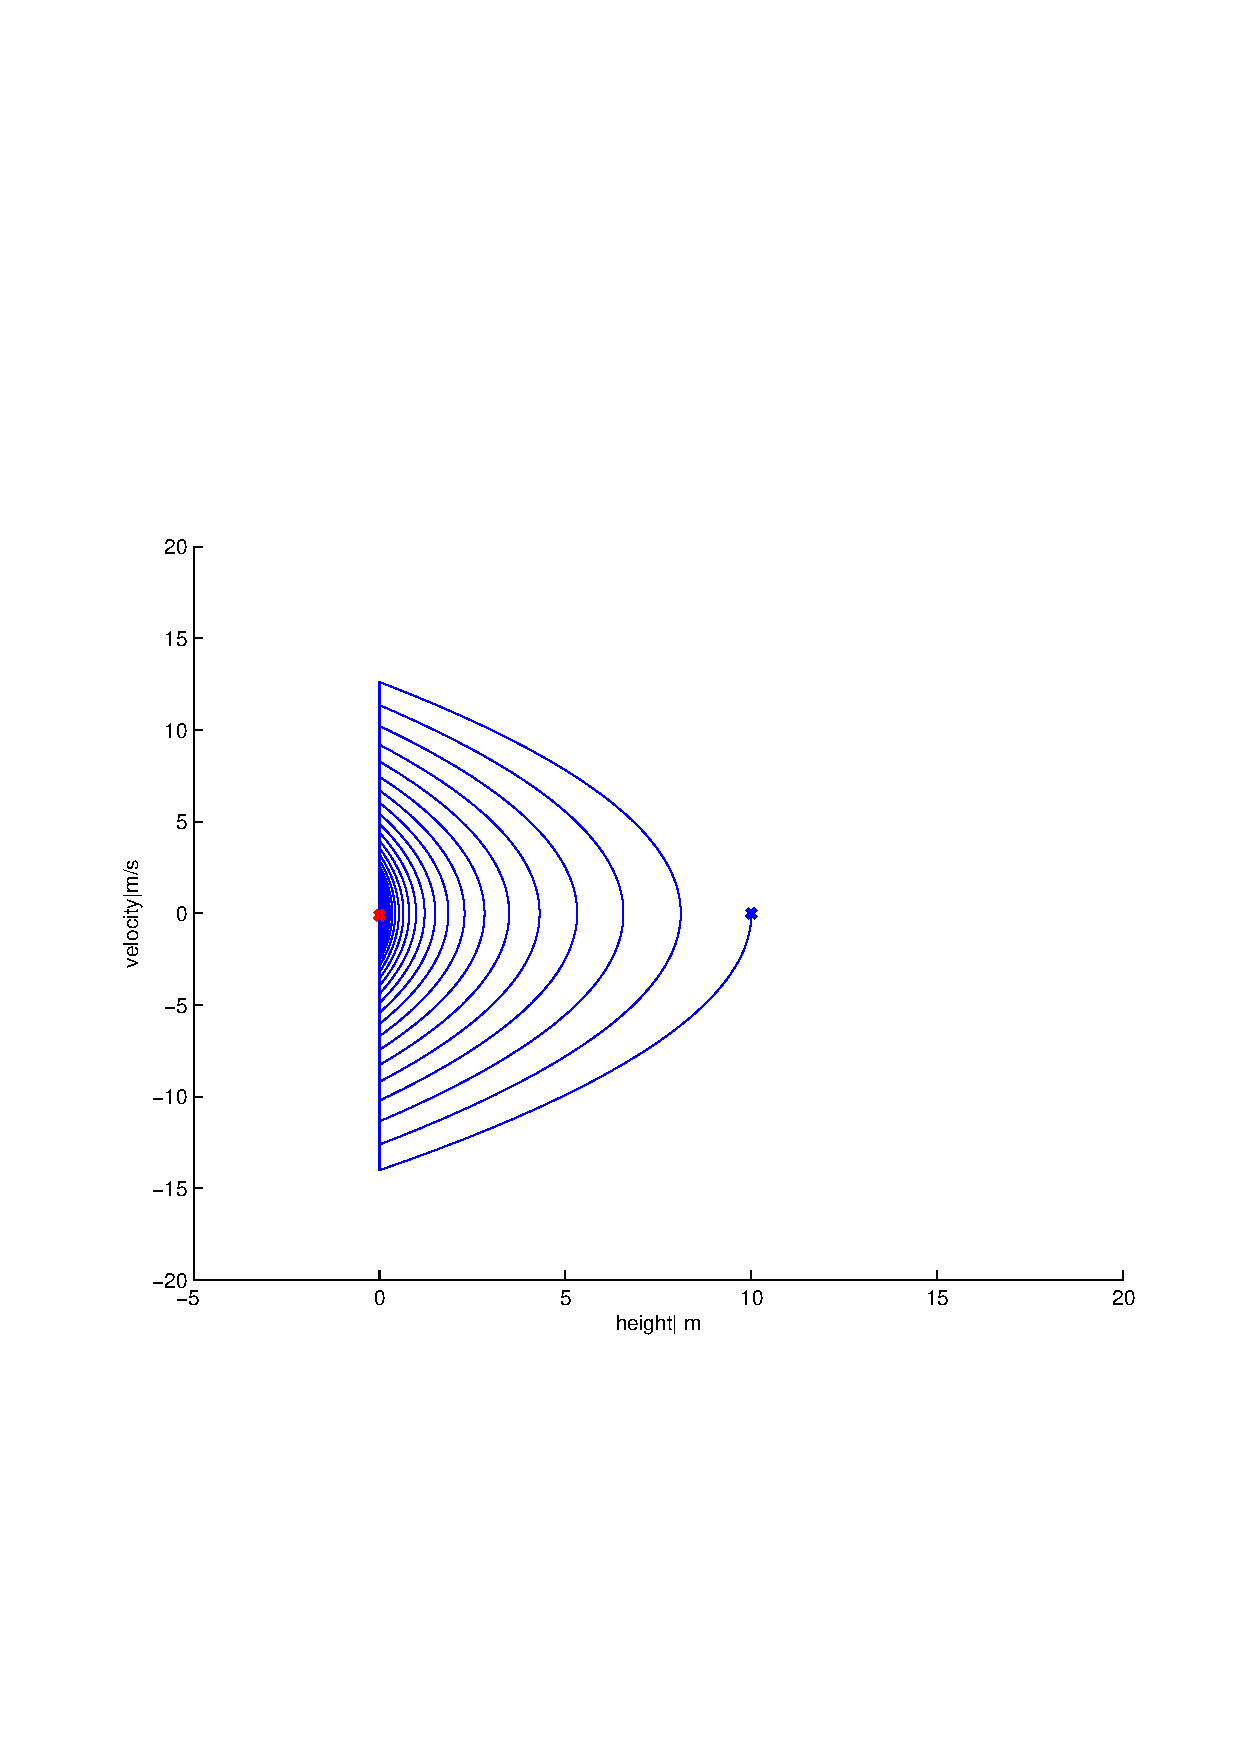
\includegraphics[width=0.7\textwidth]{BouncingBallPhasePlotuncontrolledDropAt10}
    \caption{Drop at 10}
    \label{fig:bouncing10}
\end{center}
\end{figure}




